% \usepackage{listings}
\chapter{Introduction}
\lhead{\emph{Introduction}}
This section will introduce the thesis.
\section{Smart Grids}
The energy grid is comprised of four main sectors:

        \begin{center}
            \begin{tabular}{|l |l|}
            \hline
             \textbf{Sector} & \textbf{Description} \\
             \hline\hline
             \hline
             Generation & 
             Energy is produced through either renewable or non-renewable \\ &
             sources, for example a coal burning power plant or a hydro-electric \\  &
             power producing dam. \\
             \hline
             Transportation & 
             Energy which has been produced is transmitted in high volume from \\ &
             the point of origin towards the something dense regions \\ &
             where the energy is consumed. \\
             \hline
             Distribution & 
             The power is redistributed to where the load is required along \\ &
             a local network connected to the end consumers. \\ 
             \hline
             Consumption & 
             Where the energy is consumed by the end user. \\
             \hline
            \end{tabular}
        \end{center}
In traditional power grids, the power generation comes from large centralized facilities. The power is then sent to central load centres which then directly sends power to the consumers as load requires. In a smart grid there is an unconventional power flow, meaning that the flow of power can be managed in order to redistribute it. It supports a two-way flow of information, being that utilities can send commands to the consumer as well as the end user is capable of gathering and returning information on their power consumption back to the utility. Smart grids allow for a automatic \& distributed energy delivery network.
A smart meter is a device installed on the consumer end of the energy grid. It is an advanced digital energy meter which contains information from the end user's load devices. It's capable of measuring the energy consumption of the consumer in real time. The information gathered by the smart meter can be transmitted back to the utilities. In the existing grid system, consumption monitoring is carried out manually which delays the billing process and doesn't allow for consumers to make smart decisions around their energy consumption such as using energy heavy devices during peak load times when energy is at a premium. Smart meters allow for real time consumption monitoring and automatic billing. As the communication between user and utility is bi-directional, the utility can now remotely disconnect and reconnect loads. In addition to real time monitoring, utility companies can use the data gathered to construct models to accurately forecast demand.  You can break down energy forecasting into three categories, short, medium and long term. Short term demand modelling is used to forecast energy consumption hours or days in advance. This provides valuable maintenance and operation information, for example this will determine how which power producing facilities will be required to be online for a certain time period. This type of forecasting has obvious environmental impacts as it allows energy producers to minimize the number of non-renewable power producing facilities to be active and maximizes the number of renewable power sources. Medium term forecasting is of particular interest to energy companies as it provides them with information about the market needs of energy moving forward, this will allow them to schedule fuel prices and reduce financial risk. Long term forecasting is important on a governmental level, allowing for policy makers to plan ahead. A smart meter's data could be built up of a unique identification, the electrical consumption (typically in kWh for domestic dwellings) and a time stamp. Other data can be sent back to the utility in order to diagnose detected anomalies. Value propositions for the various stakeholders. 
%https://ieeexplore-ieee-org.cit.idm.oclc.org/document/1717600
\begin{itemize}
\item The Utilities
    \begin{itemize}
    \item It saves a lot of money by improving the remote area reading and billing system
    \item It gives the ability to better manage during peak load times
    \item It makes more efficient use of energy grid resources
    \item It offers new tariff model in the electricity market
    \item It improves the transformer load management for the transmission lines
    \end{itemize}
\item The Consumers
    \begin{itemize}
    \item It shows customer data about their electricity habit
    \item It gives customer more accurate timely electricity billing
    \item It helps customer to better use the electrical equipment during the expensive hours
    \item It facilitates customer to switch/delay their electrical equipment with significant consumption to less expensive hours
    \end{itemize}
\item Governments
    \begin{itemize}
    \item It stimulates the economy by investing in smart metering networks
    \item It improves the environmental condition by reducing C02 emission
    \item It leads to reduction of consumption by increasing the awareness of consumption pattern
    \item It gives data for improving efficiency and reliability of service
    \end{itemize}
\end{itemize}

Means of generating and storing user data has evolved greatly over the past number of years, for example, through smart metering its possible to install a device to monitor and store the energy consumption of a domestic or residential property on a minute by minute basis. \\
Typically in residential setting, an analogue energy meter is installed in the premises. This meter reads the amount of energy consumed in kWh. Energy suppliers will typically send out  a technician to take a reading which then can be billed back to the consumer. In the interim between technician visits, the energy supplier could make an estimate of the energy consumption based on previous readings. Smart metering allows for the streaming of data back to the energy supplier. This removes the need for the energy supplier to schedule routine inspections. There is a big drive from Utility companies to upgrade their infrastructure and integrate more advanced tools for monitoring consumer behaviour.
For instance, the energy sector is moving towards an Intelligent Energy Network (IEN), the goal of IENs is to enable reliable, stable, secure and smart energy networks. These way this can be achieved is through incorporating new technologies and through higher integrating between existing services. There are many different focus areas of an IEN such as energy storage integration, Protection and fault calculation, Stability, Reliability \& Power quality to name a few.

%https://www.et.aau.dk/research-programmes/intelligent-energy-systems-and-active-networks/mission-and-focus-areas/ \\
% **HERE: What do we aim to do?**


        \begin{figure}[H]
        \centering     
        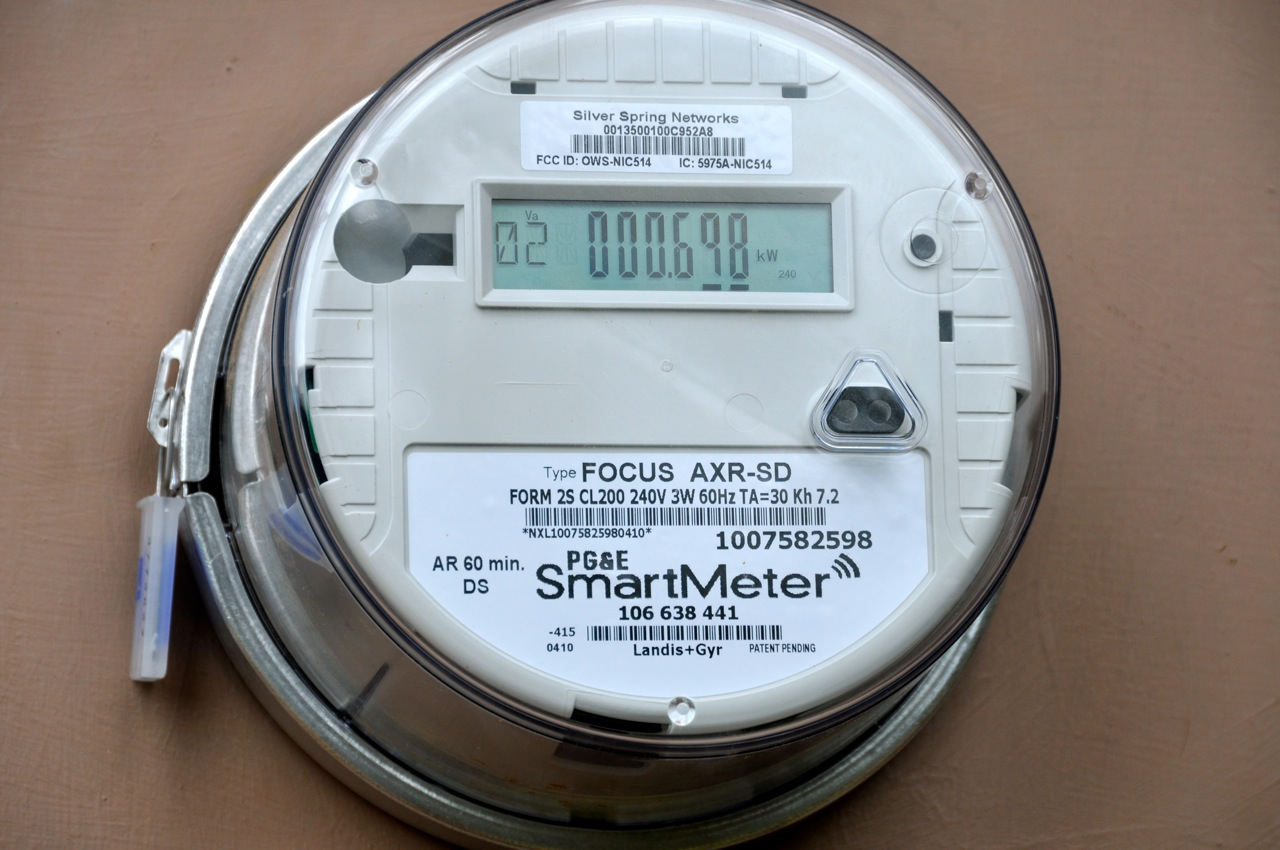
\includegraphics[width=1\textwidth]{Figures/smart-meter-emf-safety-network.jpg}
        \caption{Example of a Smart Meter}
        \label{fig:Daily Consumption}
        \end{figure}